%% Преамбула TeX-файла

% 1. Стиль и язык
\documentclass[utf8x, 12pt]{G7-32} % Стиль (по умолчанию будет 14pt)
% Остальные стандартные настройки убраны в preamble.inc.tex.
\sloppy

% Настройки стиля ГОСТ 7-32
% Для начала определяем, хотим мы или нет, чтобы рисунки и таблицы нумеровались в пределах раздела, или нам нужна сквозная нумерация.
\EqInChapter % формулы будут нумероваться в пределах раздела
\TableInChapter % таблицы будут нумероваться в пределах раздела
\PicInChapter % рисунки будут нумероваться в пределах раздела

% Добавляем гипертекстовое оглавление в PDF
\usepackage[
bookmarks=true, colorlinks=true, unicode=true,
urlcolor=black,linkcolor=black, anchorcolor=black,
citecolor=black, menucolor=black, filecolor=black,
]{hyperref}

\usepackage{graphicx}   % Пакет для включения рисунков

% Пакет Tikz
\usepackage{tikz}
\usetikzlibrary{arrows,positioning,shadows}

% Произвольная нумерация списков.
\usepackage{enumerate}


% Шрифты. Это работает только с XeLaTeX'ом
\usepackage{fontspec}
\usepackage{xunicode}
\usepackage{xltxtra}
\defaultfontfeatures{Mapping=tex-text, Scale=MatchLowercase}
\newfontfamily{\cyrillicfont}{Times}
\setmainfont{Times}
\setromanfont{Times}
%\usepackage{polyglossia}
%\setdefaultlanguage{russian}
%\setmainlanguage{russian}
%\setotherlanguage{english}

% Настройки листингов.
% 8 Листинги

\usepackage{listings}

% Значения по умолчанию
\lstset{
  basicstyle= \footnotesize,
  breakatwhitespace=true,% разрыв строк только на whitespacce
  breaklines=true,       % переносить длинные строки
%   captionpos=b,          % подписи снизу -- вроде не надо
  inputencoding=koi8-r,
  numbers=left,          % нумерация слева
  numberstyle=\footnotesize,
  showspaces=false,      % показывать пробелы подчеркиваниями -- идиотизм 70-х годов
  showstringspaces=false,
  showtabs=false,        % и табы тоже
  stepnumber=1,
  tabsize=4,              % кому нужны табы по 8 символов?
  frame=single
}

% Стиль для псевдокода: строчки обычно короткие, поэтому размер шрифта побольше
\lstdefinestyle{pseudocode}{
  basicstyle=\small,
  keywordstyle=\color{black}\bfseries\underbar,
  language=Pseudocode,
  numberstyle=\footnotesize,
  commentstyle=\footnotesize\it
}

% Стиль для обычного кода: маленький шрифт
\lstdefinestyle{realcode}{
  basicstyle=\scriptsize,
  numberstyle=\footnotesize
}

% Стиль для коротких кусков обычного кода: средний шрифт
\lstdefinestyle{simplecode}{
  basicstyle=\footnotesize,
  numberstyle=\footnotesize
}

% Стиль для BNF
\lstdefinestyle{grammar}{
  basicstyle=\footnotesize,
  numberstyle=\footnotesize,
  stringstyle=\bfseries\ttfamily,
  language=BNF
}

% Определим свой язык для написания псевдокодов на основе Python
\lstdefinelanguage[]{Pseudocode}[]{Python}{
  morekeywords={each,empty,wait,do},% ключевые слова добавлять сюда
  morecomment=[s]{\{}{\}},% комменты {а-ля Pascal} смотрятся нагляднее
  literate=% а сюда добавлять операторы, которые хотите отображать как мат. символы
    {->}{\ensuremath{$\rightarrow$}~}2%
    {<-}{\ensuremath{$\leftarrow$}~}2%
    {:=}{\ensuremath{$\leftarrow$}~}2%
    {<--}{\ensuremath{$\Longleftarrow$}~}2%
}[keywords,comments]

% Свой язык для задания грамматик в BNF
\lstdefinelanguage[]{BNF}[]{}{
  morekeywords={},
  morecomment=[s]{@}{@},
  morestring=[b]",%
  literate=%
    {->}{\ensuremath{$\rightarrow$}~}2%
    {*}{\ensuremath{$^*$}~}2%
    {+}{\ensuremath{$^+$}~}2%
    {|}{\ensuremath{$|$}~}2%
}[keywords,comments,strings]

% Подписи к листингам на русском языке.
\renewcommand\lstlistingname{Листинг}
\renewcommand\lstlistlistingname{Листинги}

% Полезные макросы листингов.
% Любимые команды
\newcommand{\Code}[1]{\textbf{#1}}


\begin{document}

\frontmatter % выключает нумерацию ВСЕГО; здесь начинаются ненумерованные главы: реферат, введение, глоссарий, сокращения и прочее.

%% Также можно использовать \Referat, как в оригинале
\begin{abstract}
Это пример каркаса расчётно-пояснительной записки, желательный к использованию в РПЗ проекта по курсу РСОИ.

Дополняет краткое пособие по графике в Latex.  Данный опус, как и более новые версии этого документа, можно взять по адресу (\url{http://sevik.ru/latex}). Минимально необходимые пакеты Latex, которые должны стоять: mathtext, amssymb, amsmath, icomma, longtable, graphicx, underscore, cmap, hyperref.

Текст в документе носит совершенно абстрактный характер.
\end{abstract}

%%% Local Variables: 
%%% mode: latex
%%% TeX-master: "rpz"
%%% End: 
 % Походу это нам не надо


% IDEF0
% USE CASE
% COMPONENTS
% SCREENSHOTS
% LIST OF TECHNOLOGIES
% Актуальность — автоматизация
% Аналоги
% Преза


\tableofcontents

\Defines % Необходимые определения. Вряд ли понадобться
\begin{description}
  \item[Облачные Технологии] (англ. cloud computing), модель обеспечения повсеместного и удобного сетевого доступа по требованию к общему пулу (англ. pool) конфигурируемых вычислительных ресурсов (например, сетям передачи данных, серверам, устройствам хранения данных, приложениям и сервисам — как вместе, так и по отдельности), которые могут быть оперативно предоставлены и освобождены с минимальными эксплуатационными затратами и/или обращениями к провайдеру.
  \item[Amazon Elastic Compute Cloud] Веб-сервис, который предоставляет вычислительные мощности в облаке. Сервис входит в инфраструктуру Amazon Web Services.
  \item[Amazon Web Services] Облачная платформа от компании Amazon, в которой представлено много сервисов для предоставления различных услуг, таких как: хранение данных, аренда виртуальных серверов, предоставление вычислительных мощностей и др.
\end{description} % Походу это нам не надо
\Abbreviations %% Список обозначений и сокращений в тексте
\begin{description}
  \item[ОС] Операционная Система
  \item[ПО] Программное Обеспечение
  \item[API] Интерфейс программирования приложений (англ. application programming interface)
  \item[AWS] Amazon Web Services
  \item[EC2] Amazon Elastic Compute Cloud

\end{description}

 % Сокращения
\Introduction
В большинстве магазинов розничной торговли есть камеры видеонаблюдения. При помощи алгоритмов компьютерного зрения, их можно использовать для получения различных статистических параметров, которые могут помочь владельцам магазинов лучше настроить бизнес процессы. Это может быть кол-во поситетелей, длина очереди, самая популярная витрина, и т.п.

Разрабатываемое в компании Cera Marketing решение позволяет полностью автоматизировать сбор данных с камер, их обработку и получение результатов.


 % Введение

\mainmatter % это включает нумерацию глав и секций в документе ниже

\chapter{Формирование требований к системе}

\section{Анализ предметной области}

Разрабатываемая в компании Cera Marketing система позволяет находить маршруты людей, моменты входа и выхода людей в определенные зоны, а также определять моменты контакта разных людей в определенных зонах. При этом, в отличии от аналогов, система способна работать с видео, снятом с обычных камер видеонаблюдения с практически любых углов. В связи с этим возникает необходимость предварительно настраивать алгоритм для каждого конкретного случая.

% Типичный процесс обработки видео состоит из нескольких этапов:

% \begin{enumerate}
%   \item подбор оптимальных параметров для алгоритма;
%   \item разметка изображения с камеры на зоны;
%   \item запуск алгоритма;
%   \item визуальная проверка качества работы алгоритма.
% \end{enumerate}


\subsection{Актуальность разработки}

Алгоритмы компьютерного зрения очень требовательные с точки зрения потребления ресурсов компьютера. Обработка 3-х часового видео на современном компьютере занимает по времени около 10 минут — это значит, что обрабатывать видео больше чем с 18 камер в день на сервере с одним процессорным ядром невозоможно. В связи с этим встает вопрос о параллельной обработке данных на нескольких компьютерах.

Для сокращения издержек и упрощения процессов поддержки физических серверов, актуально использование услуг провайдеров облачных решений. Многие компании предоставляют вычислительные мощности <<по требованию>>. Такие мощности обходятся гораздо дешевле, чем поддержка собственного дата-центра.

Однако, некоторые крупные клиенты очень скептически относятся к идее передачи данных другой компании. Им хотелось бы лицензировать ПО и использовать его самостоятельно, на собственных серверах. Таким образом, еще одной важной деталью является возможность автоматизации развертки ПО не только в облаке, но и впринципе на любых компьютерах.

\begin{figure}
  \centering
  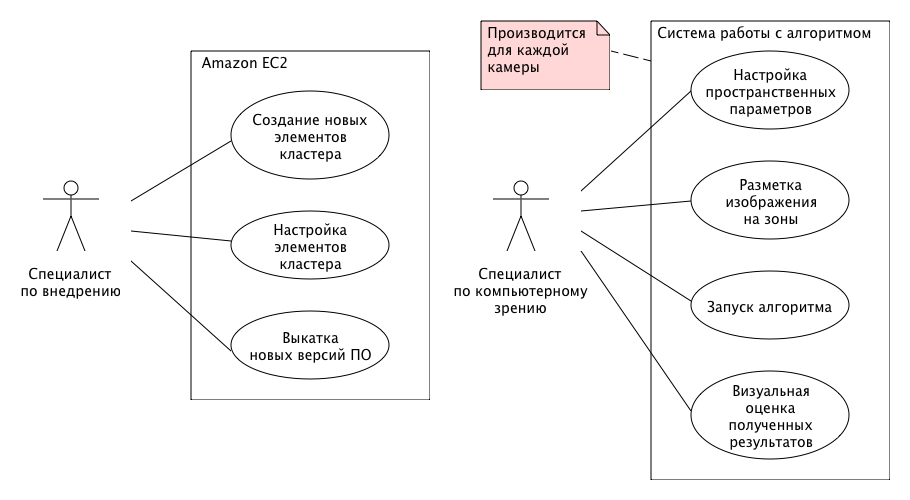
\includegraphics[width=0.8\textwidth]{assets/use-case-1.png}
  \caption{Диаграмма вариантов использования}
  \label{fig:fig01}
\end{figure}

Ко всему прочему, для каждой новой камеры параметры алгоритма необходимо подстраивать, изображение размечать на зоны, а также периодически визуально проверять качество работы. Если речь идет о нескольких видео, все это можно делать при помощи подручных средств на своем компьютере, однако если нужно работать с несколькими камерами в день встает вопрос об автоматизации процесса и передачи его в руки неподготовленного персонала.

\section{Обзор и анализ аналогов}

Прямых аналогов разрабатываемой системе не обнаружено, так как задача является очень специфической. Однако, в качестве аналогов можно рассмотривать более общие системы управления вычислительными кластерами.

\subsection{MOSIX2}
MOSIX2 — это система управления кластерами и сетями ОС на ядре Linux, представляющая их как одну систему (Single-System Image, SSI), то есть эквивалент операционной системы для кластера в целом. В кластере MOSIX2 нет необходимости в модификации существующих приложений, в связывании с дополнительными библиотеками, в явном входе на удаленные узлы — все это осуществляется автоматически на уровне ОС.

Пользователи запускают свои обычные приложения (как последовательные так и параллельные) и MOSIX прозрачно для них ищет свободные ресурсы в кластере и распределяет процессы среди доступных узлов, увеличивая тем самым общую производительность.

\subsection{MPI / Open MPI}
Программный интерфейс (API) для передачи информации, который позволяет обмениваться сообщениями между процессами. Разработан Уильямом Гроуппом, Эвином Ласком (англ.) и другими.

Базовым механизмом связи между MPI процессами является передача и приём сообщений. Сообщение несёт в себе передаваемые данные и информацию, позволяющую принимающей стороне осуществлять их выборочный приём:
\begin{enumerate}
  \item отправитель — ранг (номер в группе) отправителя сообщения;
  \item получатель — ранг получателя;
  \item признак — может использоваться для разделения различных видов сообщений;
  \item коммуникатор — код группы процессов.
\end{enumerate}
Операции приёма и передачи могут быть блокирующимися и не блокирующимися. Для не блокирующихся операций определены функции проверки готовности и ожидания выполнения операции.





% будут рассмотрены две категории аналогов — решения для анализа статистики :
% \subsection{Синезис Кассиопея}
% Видеоаналитическое решение по сбору статистики и анализу данных для бизнеса, ритейла, транспорта, общественных организаций. Бизнес-аналитика автоматически обрабатывает видеопоток с камер, анализирует видео по заданным правилам, собирает статистику и передает ее на центральный сервер.

\section{Формирование требований}

До разработки всей системы в компании Cera Marketing было произведено большое исследование потребностей клиентов, а так же исследование конкурентов.
Основными источниками требований послужили:
\begin{enumerate}
  \item представления и ожидания клиентов компании;
  \item конкурирующие программные продукты;
  % \item представления и ожидания пользователей системы;
  \item текущая организация деятельности в организации.
\end{enumerate}

\subsection{Требования к системе}

Основные требования к системе развертки:

\begin{enumerate}
  \item Возможность полной автоматической настройка ОС компьютеров кластера, а именно:
  \begin{enumerate}
    \item создание новых пользователей
    \item установка всех необходимых зависимостей
    \item установка нашего ПО
    \item базовая настройка всех компонентов ПО и зависимостей
  \end{enumerate}
  \item Автоматизация развертывание новых версий ПО:
  \begin{enumerate}
    \item обновление ПО
    \item настройка всех компонентов
    \item миграция базы данных
    \item установка новых зависимостей
  \end{enumerate}
  \item Управление элементами кластера в системе Amazon EC2, а именно:
  \begin{enumerate}
    \item запуск, остановка элементов кластера
    \item создание, удаление элементов кластера
    \item клонирование элементов кластера
  \end{enumerate}
\end{enumerate}

Требования к системе управления кластером:
\begin{enumerate}
  \item Возможность настройки пространственных параметров алгоритма
  \item Разметка картинки с камеры на зоны
  \item Запуск обработки видео
  \item Визуальная оценка качества полученных результатов
\end{enumerate}

\subsection{Требования к ПО пользователей}
Система должна работать на компьютерах под управлением всех из нижеперечисленных ОС:
\begin{enumerate}
  \item Любая ОС на базе Linux;
  \item Windows XP или выше;
  \item Mac OS X.
\end{enumerate}

и всех из нижеперечисленных браузеров:
\begin{enumerate}
  \item Google Chrome версии 6.0 или выше;
  \item Mozilla Firefox версии 4.0 или выше;
\end{enumerate}

Система развертки может быть более требовательна к ПО, установленному у пользователя, так как эта система расчитана на технически более подготовленного пользователя, однако она также должна работать на всех вышеперечисленных ОС.

В части требований к серверами, система развертки должна уметь разворачивать кластер на любых компьютерах под управлением ОС Linux.

% Обзор источников информации для требовании, формирование требовании, их обоснование (SADT, IDEF3, DFD, UML),
% анализ и пересмотр с обоснованием их правильности, текстовые сценарии использования.

\section{Постановка задачи}

В рамках данной работы необходимо спроектировать и разработать систему развертки и управления кластером в соответствии с требованиями описаными выше.



% Задачи у системы развертывания следующие:

% 1) Полная автоматическая настройка ОС компьютеров кластера, а именно:
% - создание новых пользователей
% - установка всех необходимых зависимостей
% - установка нашего ПО
% - базовая настройка всех компонентов ПО и зависимостей

% 2) Развертывание новых версий ПО
% - обновление ПО
% - настройка всех компонентов
% - миграция базы данных
% - установка новых зависимостей

% 3) Управление элементами кластера в системе Amazon Elastic Compute Cloud, а именно:
% - запуск, остановка компьютеров кластера
% - создание, удаление компьютеров кластера
% - клонирование элементов кластера


% Возможно, в ближайшем будущем к задачам системы развертывания добавятся:
% - автоматическое создание / удаление элементов кластера в зависимости от общей нагрузки на кластер (если нечего обрабатывать, зачем держать машины запущенными)
% - автоматизация тестирования новых версий нашего ПО в кластере (сейчас тестировние происходит у нас на компьютерах, занимает много времени и децентрализовано)


% Таким образом, эта система позволяет на любом кол-ве машин под управлением ОС Linux удаленно настроить вычислительный кластер, развертывать на нем наше ПО.
% В данный момент мы используем Amazon Elastic Compute Cloud, и средства управления кластером привязаны к ней. Возможно вскоре мы перейдем на что то другое, например, на выделенные сервера в дата-центре и появятся какие то другие интересные задачи, с этим связанные.


% Сейчас мы запускаем пилотный проект, в рамках которого предполагается обрабатывать видео с 10 камер. Если он окажется успешным, мы будем постепенно расширять кол-во используемых камер до 2000, а значит, появятся новые интересные трудности и проблемы, связанные с развертыванием кластера и его эффективной работой, которые я буду решать.


% Спасибо,
% Дмитрий




% Здравствуйте, Максим Валерьевич.


% Я буквально на прошлой неделе устроился в компанию CERAmarketing.

% Пока, тема того, чем я занимаюсь звучит примерно так:
% «Разработка инфраструктуры для управления вычислительным кластером в облаке»


% Описание объекта автоматизации
% В большинстве магазинов розничной торговли есть камеры видеонаблюдения. При помощи алгоритмов компьютерного зрения, их можно использовать для получения различных статистических параметров, которые могут помочь владельцам магазинов лучше настроить бизнес процессы. Это может быть длина очереди, самая популярная витрина, и т.п. Наша система позволяет полностью автоматизировать сбор данных с камер, их обработку и получение результатов.


% Функциональное назначение системы.
% Система должна через интернет захватывать видео с камер видеонаблюдения, расположенных в магазинах розничной торговли, обрабатывать его и генерировать отчеты.


% Аналоги
% Камеры со встроенным интелектом. Наше же решение позволяет использовать обычные камеры, таким образом, экономя компаниям крупные суммы денег.


% Используемые технологии:
% * Amazon AWS
% * Python
% * MySQL


% Связь автора работы с объектом автоматизации
% Я создаю систему развертывания и управления кластером, а также вэб-интерфейс для обучения системы.


% Это мои задачи на ближайшее время. Потом возможно появится что то еще.

\chapter{Проектирование системы}

\section{Системная архитектура}

Кластер — это группа компьютеров, объединённых высокоскоростными каналами связи и представляющая с точки зрения пользователя единый ресурс. Это значит, что для создания кластера необходимы как минимум несколько компьютеров. В последнее время, популярными становятся услуги облачных вычислений. Потребителю таких услуг не нужно беспокоиться о настройке физических серверов, поддержке сети и прочих аппаратных проблемах. В качестве провайдера таких услуг был выбран самый популярный подобный сервис — Amazon Elastic Compute Cloud. Доступ к системе предоставляется через API. Он позволяет создавать виртуальные машины, клонировать существующие. Есть возможность выбора разных конфигураций виртуальных машин.


\begin{figure}
  \centering
  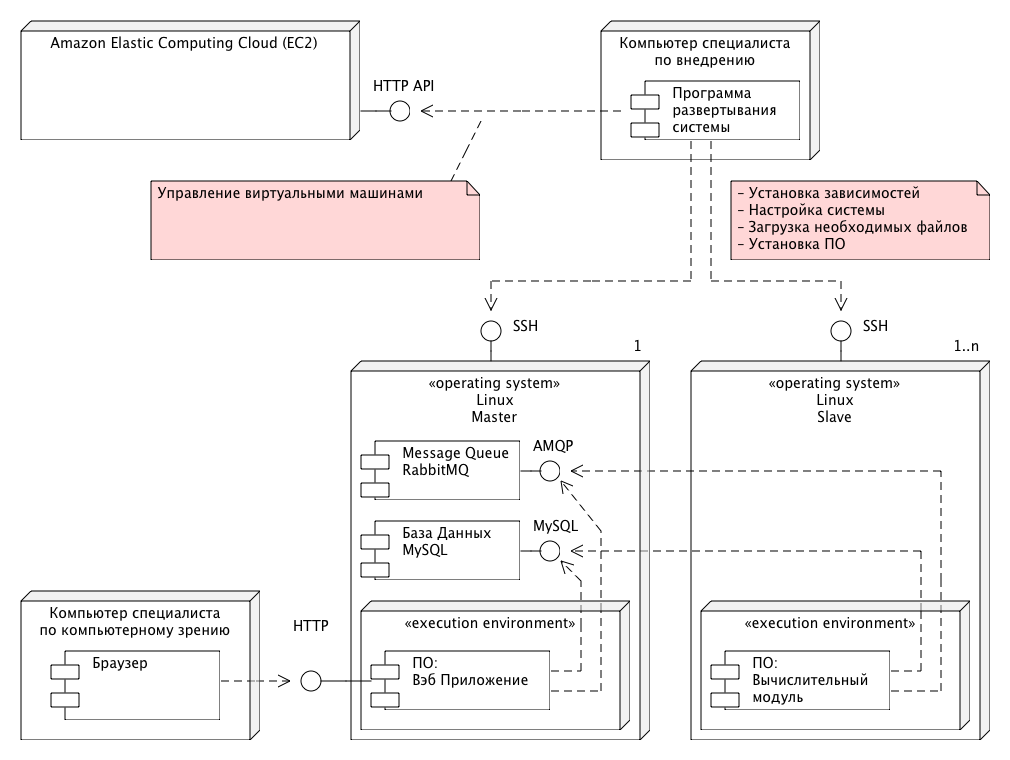
\includegraphics[width=0.8\textwidth]{assets/deploy-1.png}
  \caption{Диаграмма развертки}
  \label{fig:fig01}
\end{figure}


\section{Программная архитектура}

Классификация параллельных архитектур по Флинну определяет 4 типа параллельных систем:
\begin{enumerate}
  \item ОКОД — одиночный поток команд и одиночный поток данных;
  \item ОКМД — одиночный поток команд и множественный поток данных;
  \item МКОД — множественный поток команд и одиночный поток данных;
  \item МКМД — множественный поток команд и множественный поток данных.
\end{enumerate}

Наша система относится к 4-ому типу — вычислительная система со множественным потоком команд и множественным потоком данных.

Основными типами кластеров являются:
\begin{enumerate}
  \item Кластеры высокой доступности (High-availability clusters) — этот тип кластеров используется в случае, когда нужно обеспечить максимальную доступность сервиса. Доступность обеспечивается кол-вом серверов. Чем больше кол-во серверов, тем доступнее предоставляемый сервис.
  \item Кластеры распределения нагрузки — основная задача этого типа кластеров — повышение производительности и надежности системы путем распределении нагрузки между большим кол-вом узлов.
  \item Вычислительные кластеры — основная задача этих кластеров — быстрые вычисления. Надежность и доступность в этом случае играет маленькую роль и на первый план выходит производительность системы и удельная стоимость вычислительных ресурсов.
\end{enumerate}

По типу организации кластеров, их можно разделить на системные и программные. В первом случае объединение в один ресурс происходит на уровне ядра операционной системы. Такие системы могут перемещать процессы вместе с памятью между ядрами. Во втором случае объединение серверов в один ресурс происходит на уровне программных протоколов.

В нашем случае, разрабатываемая система является типичным примером вычислительного кластера. Мною был выбран программный подход нежели чем параллелизация на уровне ядра, по причине большей простоты и гибкости такого решения.



%Beowulf

%Диаграмма компонентов
%диаграммы UML, схемы алгоритмов.


\section{Архитектура данных}

% ERM - инфологическая
%  - диаграммы ER, инфологическая модель и даталогическая
% модель, описание основных транзакции с указанием специфичных запросов,
% хранимых процедур и триггеров.

\begin{figure}[h]
  \centering
  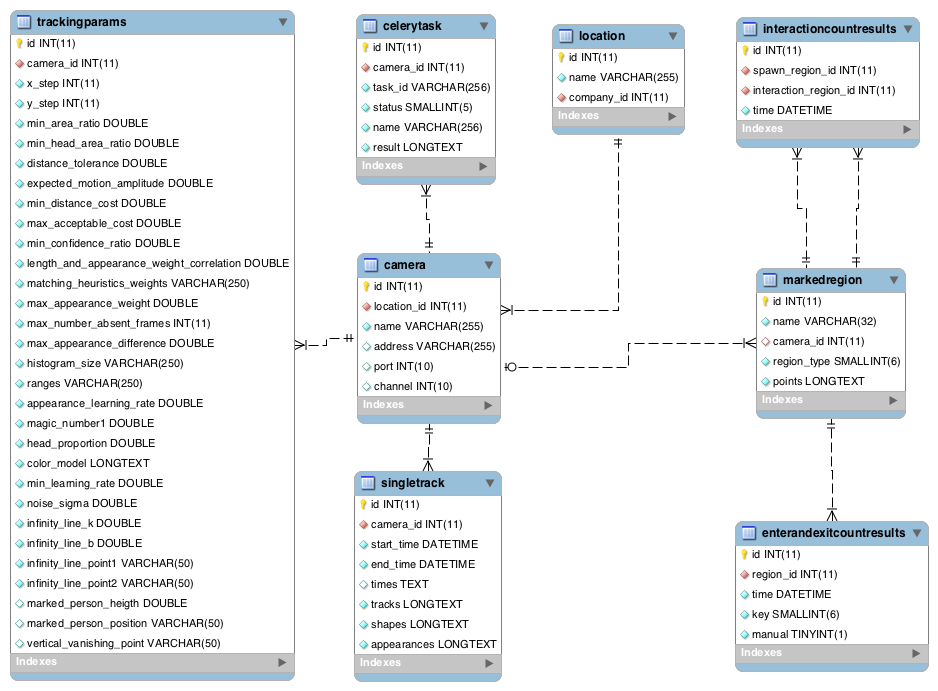
\includegraphics[width=0.8\textwidth]{assets/schema-1.png}
  \caption{Инфологическая EER модель}
  \label{fig:fig01}
\end{figure}

\chapter{Разработка системы}
%3. Материалы главы 3 пояснительнои записки. Материалы могут быть представлены не в полном объеме. Обязательным является наличие пункта Технологические особенности реализации системы.

\section{Технологические особенности реализации системы}

\subsection{Выбор программных средств}

В качестве основного языка программирования выбран Python. Python очень популярен среди ученых и, в частности, среди специалистов по компьютерному зрению.

Некоторые скрипты для установки и обновления ПО будут написаны на языке Bash, так как это основной язык, используемый для автоматизации задач в среде UNIX.

\begin{figure}[h]
  \centering
  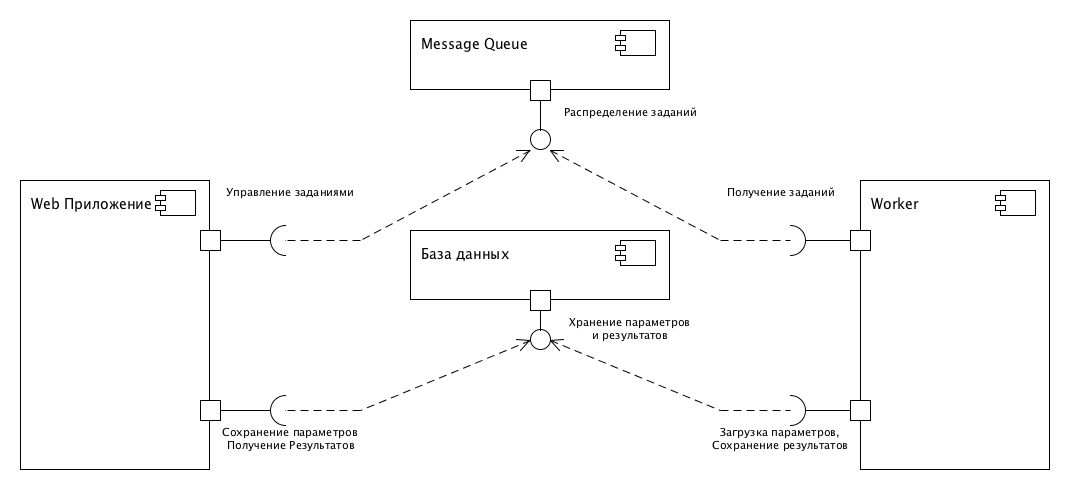
\includegraphics[width=1\textwidth]{assets/components-1.png}
  \caption{Компоненты системы}
  \label{fig:fig01}
\end{figure}



\section{Пользовательский интерфейс}

\subsection{Интерфейс системы развертки}

Поскольку работать с системой развертки будут опытные пользователи, в качестве интерфейса для этой программы предлагается интерфейс командной строки.

\subsection{Интерфейс системы управления кластером }

Пользовательский интерфейс системы управления кластером было решено сделать с применением web-технологий: HTML5, Java Script и CSS Использование web-технологий позволит быстро и просто создавать необходимые интерфейсы, а также делает решение более привычным для неподготовленных пользователей. На стороне сервера используется web-фреймворк Django - популярное решение в среде программистов на Python. Современный уровень развития web-технологий позволяет создавать полноценные кросс-платформенные интерфейсы.

Основные интерфейсы представлены ниже:
\begin{figure}[h]
  \centering
  % \fbox{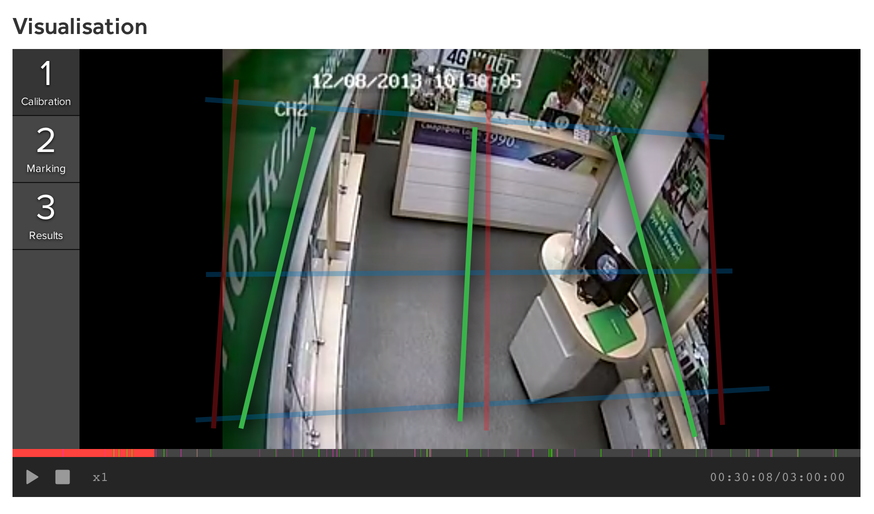
\includegraphics[width=0.8\textwidth]{assets/interface-1.png}}
  \fbox{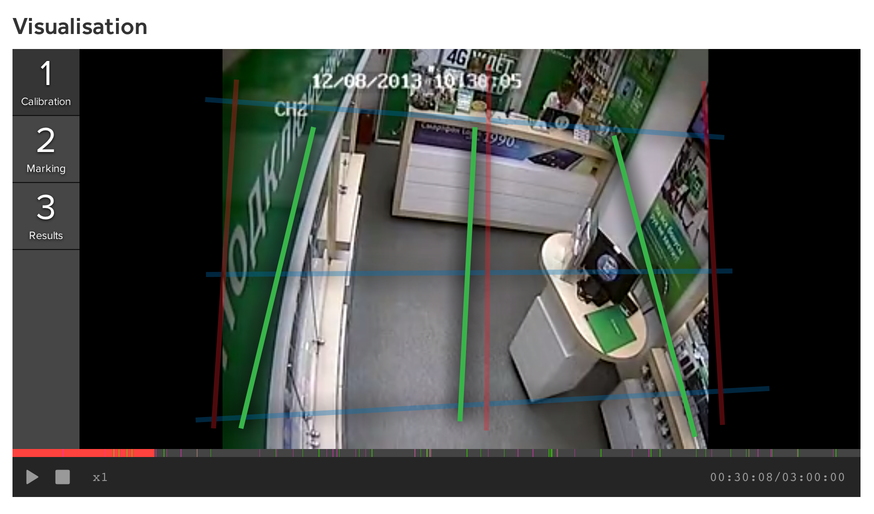
\includegraphics[width=0.8\textwidth]{assets/interface-1.png}}
  \caption{Интерфейс настройки пространственных параметров}
  \label{fig:fig01}
\end{figure}

На рисунке \ref{fig:fig01} показан интерфейс настройки пространственных параметров. Пользователю предлагается нарисовать по 3 линии в 3-х проекциях. Эта информация затем будет использована алгоритмом слежения для корректирования изображения.

\begin{figure}[h]
  \centering
  % \fbox{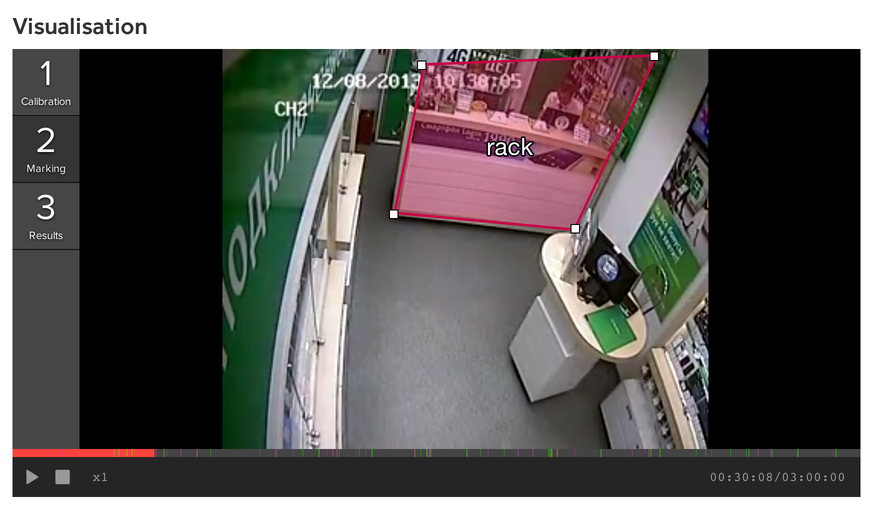
\includegraphics[width=0.8\textwidth]{assets/interface-2.png}}
  \fbox{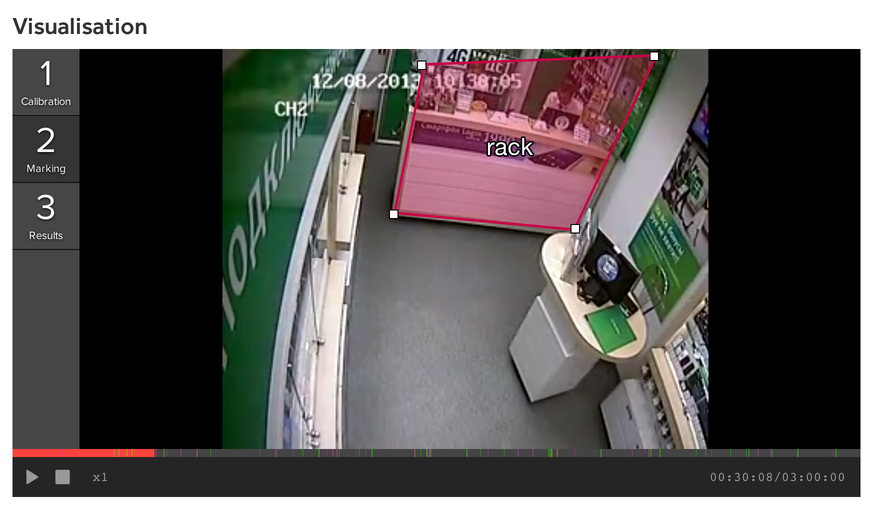
\includegraphics[width=0.8\textwidth]{assets/interface-2.png}}
  \caption{Интерфейс разметки на зоны}
  \label{fig:fig02}
\end{figure}

Для определения пересечения тракторий людей с некоторыми зонами, эти зоны необходимо сначала определить. Для этого пользователю предлагается нарисовать эти зоны на изображении (рис. \ref{fig:fig02}).

\begin{figure}[h]
  \centering
  % \fbox{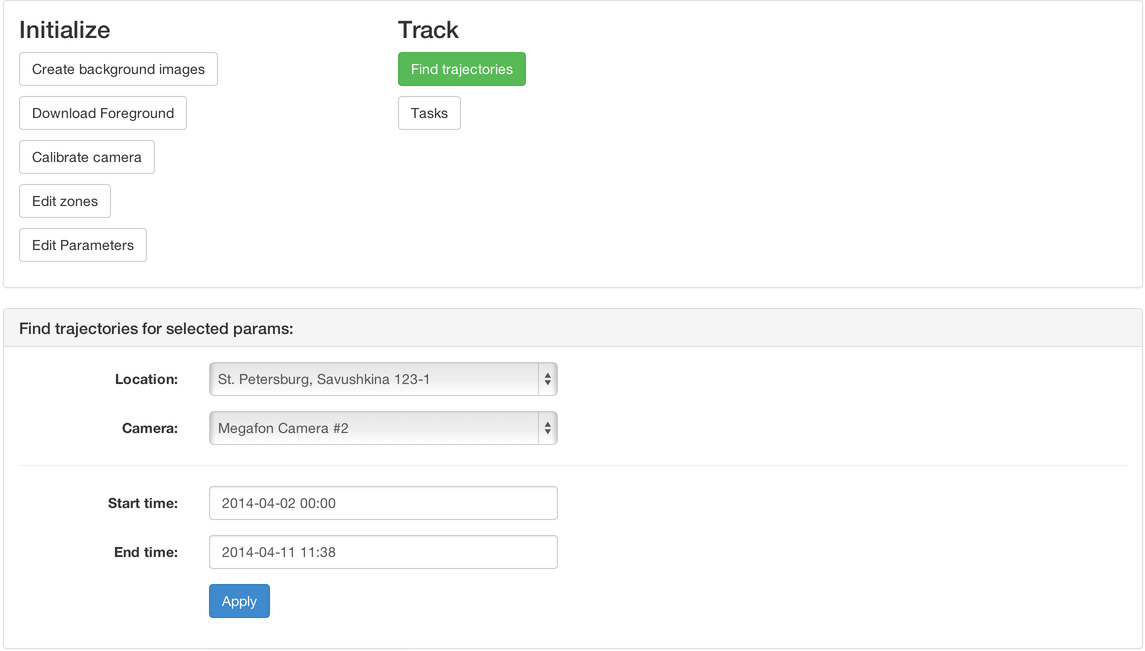
\includegraphics[width=0.8\textwidth]{assets/interface-0.png}}
  \fbox{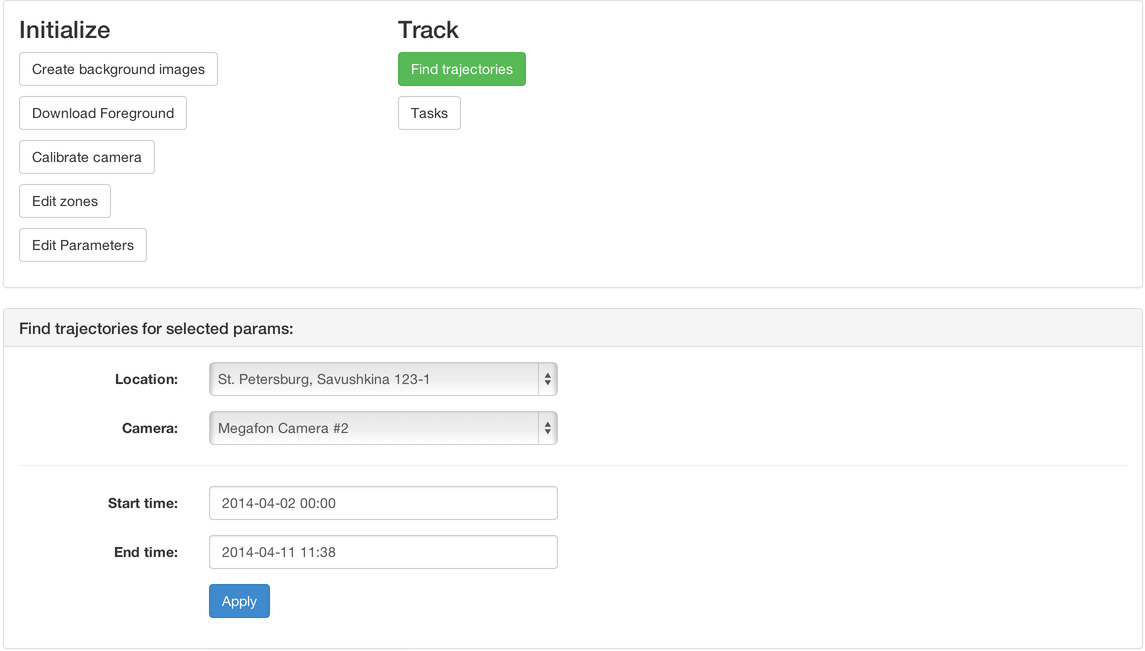
\includegraphics[width=0.8\textwidth]{assets/interface-0.png}}
  \caption{Интерфейс управления заданиями}
  \label{fig:fig03}
\end{figure}

После того, как предварительный этап закончен, можно запускать алгоритм слежения. Пользователю предлагается выбрать нужную камеру и временной период, видео в котором нужно обработать (рис. \ref{fig:fig03}).

\begin{figure}[h]
  \centering
  % \fbox{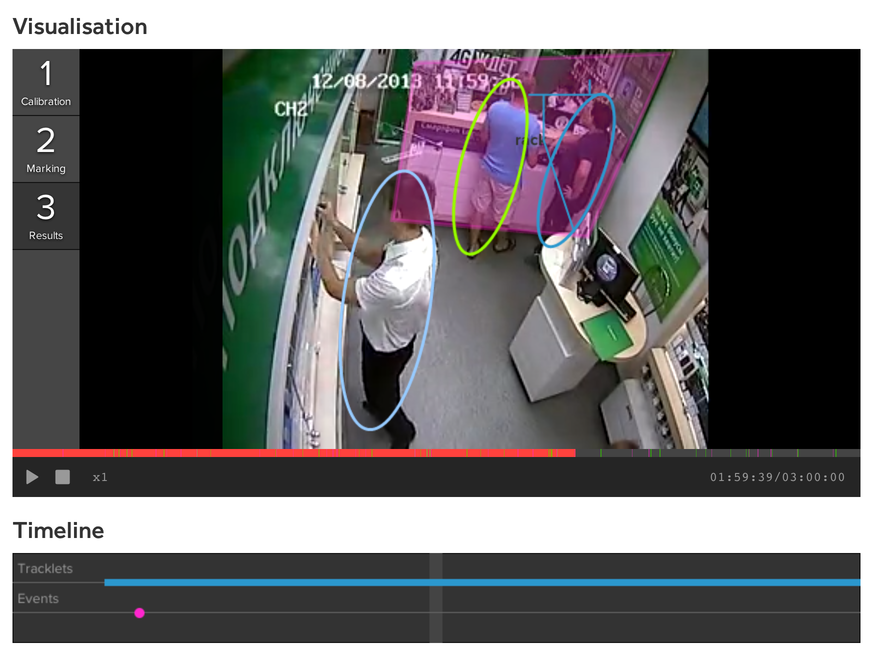
\includegraphics[width=0.8\textwidth]{assets/interface-3.png}}
  \fbox{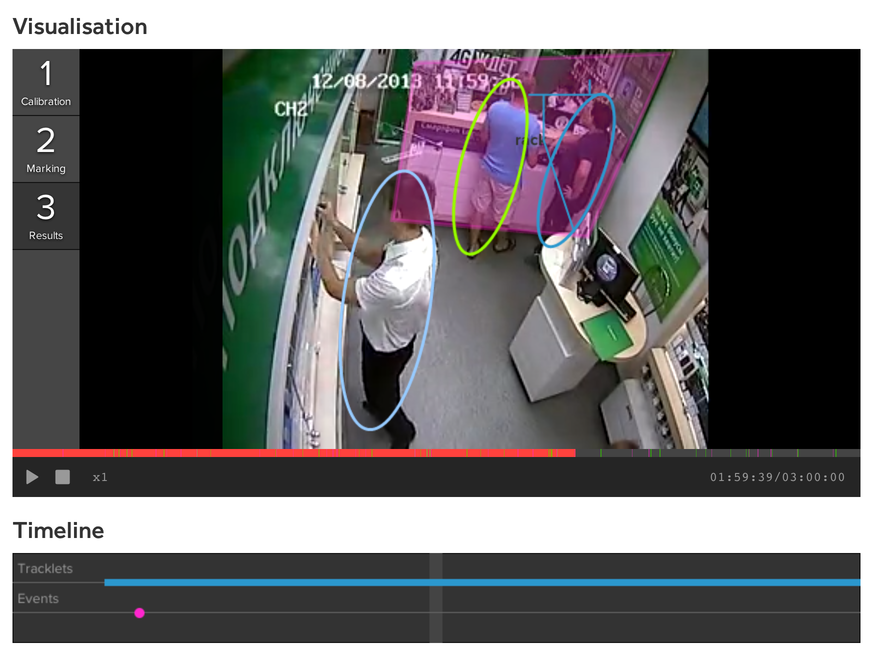
\includegraphics[width=0.8\textwidth]{assets/interface-3.png}}
  \caption{Интерфейс просмотра результатов}
  \label{fig:fig04}
\end{figure}

После того, как алгоритм закончил работу можно посмотреть результаты, для этого пользователю предлагается просмотр видео и отмеченными на нем ключевыми моментами, такими как входы и выходы из зон (рис. \ref{fig:fig04}).



%\section{План тестирования}

%\include{50-economics}
%\include{60-obz}

\backmatter %% Здесь заканчивается нумерованная часть документа и начинаются ссылки и заключение

%\Conclusion % заключение к отчёту

В результате проделанной работы стало ясно, что ничего не ясно...

%%% Local Variables: 
%%% mode: latex
%%% TeX-master: "rpz"
%%% End: 

%% % Список литературы при помощи BibTeX
% Юзать так:
%
% pdflatex rpz
% bibtex rpz
% pdflatex rpz

\bibliographystyle{gost780u}
\bibliography{rpz}

%%% Local Variables:
%%% mode: latex
%%% TeX-master: "rpz"
%%% End:


%\appendix   % Тут идут приложения

%\chapter{Картинки}
\label{cha:appendix1}

\begin{figure}
\centering

\includegraphics[width=\textwidth]{assets/cage.jpg}
\caption{Картинка в приложении. Страшная и ужасная.}
\end{figure}

%%% Local Variables:
%%% mode: latex
%%% TeX-master: "rpz"
%%% End:

%\chapter{Еще картинки}
\label{cha:appendix2}

\begin{figure}
\centering

\includegraphics[width=\textwidth]{assets/cage.jpg}
\caption{Еще одна картинка, ничем не лучше предыдущей. Но надо же как-то заполнить место.}
\end{figure}

%%% Local Variables:
%%% mode: latex
%%% TeX-master: "rpz"
%%% End:


\end{document}

%%% Local Variables:
%%% mode: latex
%%% TeX-master: t
%%% End:
